 \subsection{Patient Data Adjudication and EGM Template Extraction}
In order to obtain realistic \ac{EGM} morphologies for our simulations we utilize the Ann Arbor Electrogram Libraries (AAEL), a database of over 500 \ac{EGM} recordings from real patients made during clinical electrophysiology studies~\cite{AAEL}. 
The AAEL is used by all major \ac{ICD} manufacturers and is licensed by the US FDA. 
123 records from 47 patients were manually examined and adjudicated into segments called \emph{episodes} containing one specific rhythm, e.g.\, \ac{NSR}, \ac{VF}, etc. 
The adjudication was performed by an experienced cardiologist.
We developed an automated process which extracted \ac{EGM}s from a given episode. 
The \acp{EGM} are collected and organized by both patient and by the type of rhythm which was annotated during the adjudication process.
These extracted \acp{EGM} are used in the morphology model described in the previous section to create the signals.
%Fig. \ref{fig:adjudication} (right) depicts an example of 10 signatures extracted from the record. 

%\begin{figure*}[t]
%	\centering
%	\vspace{-10pt}
%	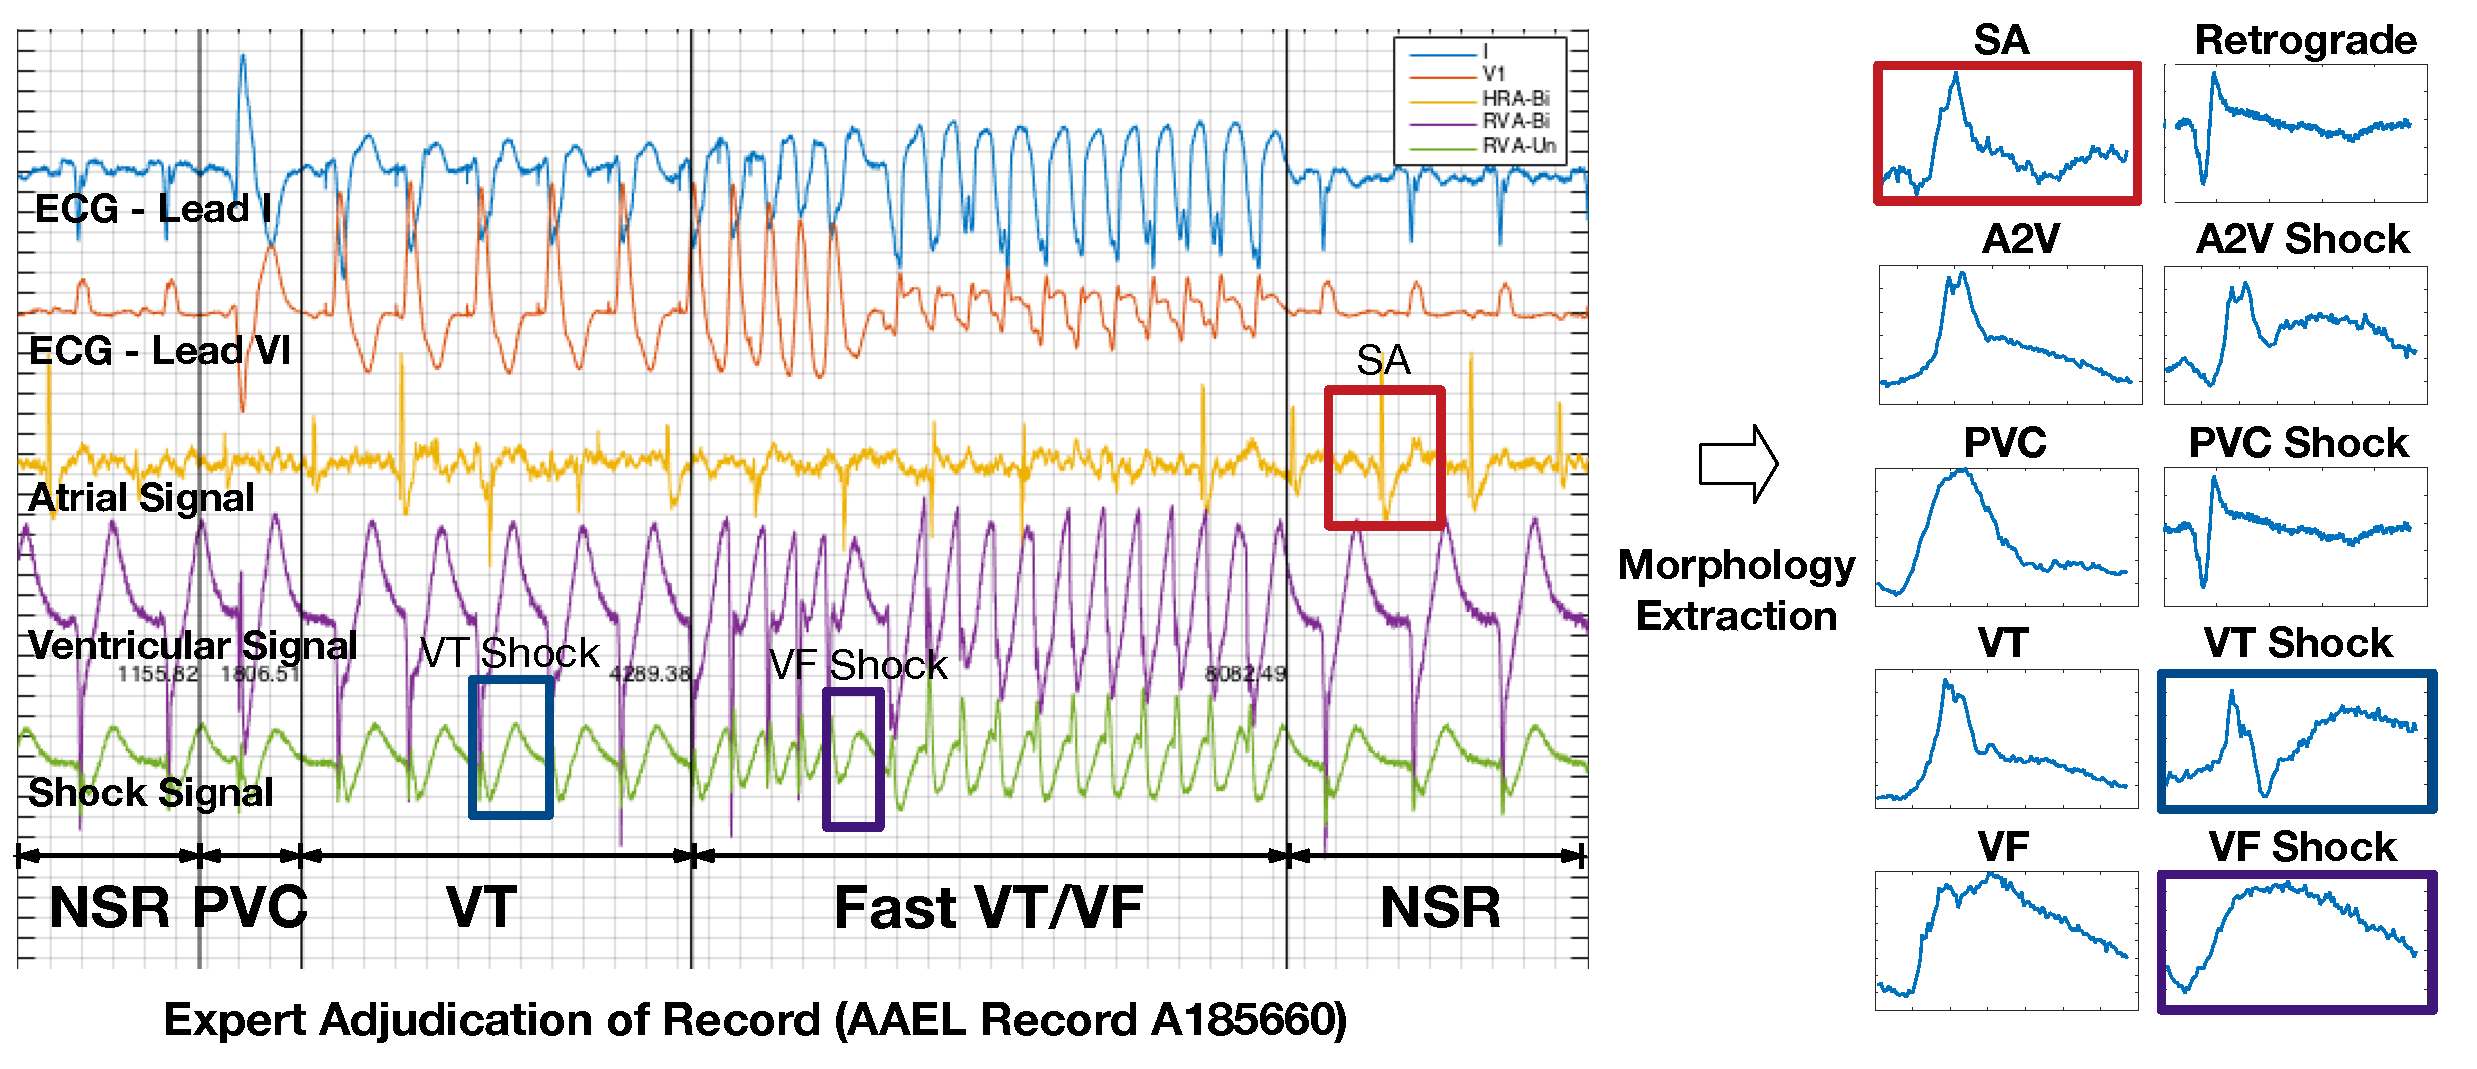
\includegraphics[scale=0.35]{figures/figAdjudication.pdf}
%	\vspace{-10pt}
%	\caption{\small  (Left) The \ac{EGM} record is segmented into episodes with distinct rhythms in each. (Right) From each episode, individual \acp{EGM} morphologies are extracted and stored.
%	}
%	\label{fig:adjudication}
%\end{figure*}
